%
% ACM Engage course material
%
%<*acmengage>
%%
%% 
%% Commands for TeXCount
%<<TCMACROS
%TC:macro \cite [option:text,text]
%TC:macro \citep [option:text,text]
%TC:macro \citet [option:text,text]
%TC:envir table 0 1
%TC:envir table* 0 1
%TC:envir tabular [ignore] word
%TC:envir displaymath 0 word
%TC:envir math 0 word
%TC:envir comment 0 0
%TCMACROS
%% 
%% 
%% The first command in your LaTeX source must be the \documentclass command.

\documentclass[sigconf]{acmart}

%% \BibTeX command to typeset BibTeX logo in the docs
\AtBeginDocument{%
  \providecommand\BibTeX{{%
    Bib\TeX}}}

%% Rights management information.  This information is sent to you
%% when you complete the rights form.  These commands have SAMPLE
%% values in them; it is your responsibility as an author to replace
%% the commands and values with those provided to you when you
%% complete the rights form.  Note that by default course materials
%% use Creative Commons license
%

\usepackage{tikz}
\usepackage{enumitem}
\usetikzlibrary{positioning, arrows.meta}

\setcopyright{cc}
\setcctype{by}
\copyrightyear{2026}
\acmYear{2026}
\acmConference[BID '26]{Benchmarking in the Data Center}{September 28, 2026}{Singapore}
\acmBooktitle{Benchmarking in the Data Center (BID '26), September 28, 2026, Singapore}
\acmDOI{XXXXXXX.XXXXXXX}

\begin{document}
\title{Less is More: Optimising SGLang Distributed DeepSeek-R1 Inference on a Two-Node H200 Cluster}
\author{Luca Lowndes}
\email{luca@lowndes.net}
\affiliation{%
    \institution{Monash University}
  \city{Melbourne}
  \country{Australia}}

\author{Nathan Culshaw}
\email{nathanculshaw2@gmail.com}
\affiliation{%
  \institution{Monash University}
  \city{Melbourne}
  \country{Australia}}

% \author{Author Three}
% \email{author3@school.xxx}
% \affiliation{%
%   \institution{A3 affiliation}
%   \city{SomeCity}
%   \country{SomeCountry}}

%% The synopsis is a name for the abstract
\begin{abstract}
For an operator holding a fixed GPU allocation, the question is not whether a frontier open-source model can be served, but how many tokens per second the hardware can produce. This paper reports a throughput-maximisation campaign for offline inference of DeepSeek-R1 (671B parameters, 37B active per token) using SGLang 0.5.3rc1 on two 8-GPU H200 nodes, under a fixed benchmark of 2,000 ShareGPT prompts at BF16 precision. From the two-node baseline of 9,610.57 tok/s (TP=16), a pinned container image, runtime compilation, and a hybrid parallelisation of TP=4, DP=4, PP=2 with data-parallel attention raised the best run to 17,417.40 tok/s, an 81.2\% improvement using only the eight GPUs of a single node. Every layout whose per-layer collectives crossed the InfiniBand fabric was beaten by one that kept them on NVLink: the best engine spanning both nodes reached 17,032.39 tok/s while idling half its GPUs, and a 40-configuration NCCL sweep found no manual setting that outperformed the library's autotuned defaults, indicating the internode penalty is physical rather than a misconfiguration. Per GPU, the tuned single node delivers 2.05$\times$ the throughput of the best two-node engine. For multi-node serving we therefore recommend replication over distribution: a half-workload run projects two independent single-node replicas at a combined 23,773.58 tok/s, 39.6\% above the best distributed engine. At this model scale and on this class of interconnect, less is more.

% This paper builds upon current distribution methods with novel insights  

\end{abstract}

%% CCS Concepts (required by ACM). Verify/regenerate the XML at https://dl.acm.org/ccs
%% then paste the generated block here if the concept IDs differ.
\begin{CCSXML}
<ccs2012>
 <concept>
  <concept_id>10002944.10011122.10011126</concept_id>
  <concept_desc>General and reference~Performance</concept_desc>
  <concept_significance>500</concept_significance>
 </concept>
 <concept>
  <concept_id>10010520.10010521.10010537</concept_id>
  <concept_desc>Computer systems organization~Distributed architectures</concept_desc>
  <concept_significance>300</concept_significance>
 </concept>
 <concept>
  <concept_id>10010147.10010257</concept_id>
  <concept_desc>Computing methodologies~Machine learning</concept_desc>
  <concept_significance>100</concept_significance>
 </concept>
</ccs2012>
\end{CCSXML}

\ccsdesc[500]{General and reference~Performance}
\ccsdesc[300]{Computer systems organization~Distributed architectures}
\ccsdesc[100]{Computing methodologies~Machine learning}

%% Keywords
\keywords{DeepSeek-R1, Inference Parallelism, H200, SGLang, Attention}
\maketitle

\section{Introduction}
Large language model (LLM) inference has become a dominant data-centre workload, a workload that GPUs are at the centre of.

For distributed training, the trade-offs are well documented. Tensor, Pipeline and Data Parallelism have precise, extensively studied cost models. High-throughput inference of very large mixture-of-experts (MoE) models has no such consensus, especially at smaller scales, where popular throughput maximisation techniques don't pay off. Serving frameworks expose dozens of interacting knobs: parallelism layouts, memory policies, CUDA-graph capture limits, communication-library tuning, container runtimes. Guidance is largely written for hyperscale deployments spanning tens if not hundreds of nodes. For the one-to-two node allocations that most research groups and national facilities actually grant, guides on throughput optimisations are spread thin.

This paper explores a throughput-maximisation campaign that seeks to uncover the optimal configuration for deploying DeepSeek-R1 \cite{deepseekr1}, a 671B-parameter MoE reasoning model with 37B active parameters per token, using SGLang on two NVIDIA H200 nodes, under a fixed offline benchmark protocol (Section 3.3): 2,000 ShareGPT prompts, BF16 precision, and a fixed random seed.

Starting from the baseline two-node deployment of 9,610.57 tok/s (TP=16), we reach a best measured run of 17,417.40 tok/s on a single node, an 81.2\% improvement. The gains decompose into a pinned container stack, runtime compilation, and above all a hybrid parallelisation (TP=4, DP=4, PP=2 with data-parallel attention) that trades communication for KV-cache capacity. Our investigation found every configuration whose per-layer collectives crossed the InfiniBand fabric ($\approx$46 GB/s per adapter) was outperformed by one that kept them on NVLink (478 GB/s). Even the best two-node engine we could construct was the same hybrid layout spanning the fabric only at one layer boundary across all 61 transformer blocks, reaching 17,032.39 tok/s while leaving half of its sixteen GPUs idle. \emph{Our contributions are:}
\begin{itemize}[nosep]   
  \item A decomposition of the 1.81$\times$ throughput improvement into its individual configuration decisions: container stack, parallelism layout, runtime compilation, and (for the TP=16 layout only) scheduler memory policy.
  \item An in-depth explanation as to why TP=4, DP=4, PP=2 with data-parallel attention is the right shape for DeepSeek-R1 on an 8-GPU node.
  \item A sweep of 40 NCCL configurations in which no manual setting outperformed NCCL's autotuned defaults, evidence that the internode penalty is physical rather than a software misconfiguration.
  \item Deployment guidance for MoE inference at modest scale: exhaust a single node before spanning two, avoid distributing one engine where possible, and if an engine must span nodes, use pipeline parallelism to do it.
\end{itemize}
The benchmark was fixed as part of the 2025 APAC HPC-AI Competition~\cite{apachpcai2025}.

\section{Background}

\begin{figure}
    \centering
    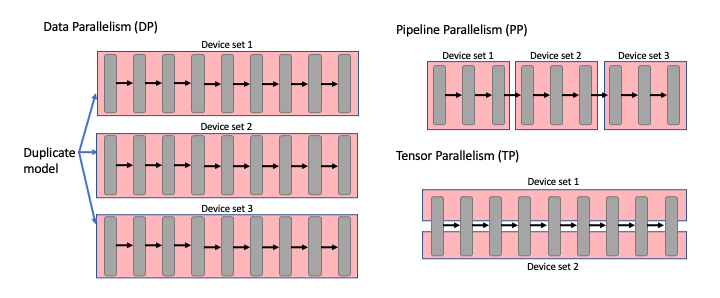
\includegraphics[width=1\linewidth]{parallelismTechniques.png}
    \caption{Depiction of Data Parallelism (DP), Pipeline Parallelism (PP), and Tensor Parallelism (TP). Models are duplicated across devices in DP, broken into sequential stages spread across devices in PP, and individual layers are split across devices in TP.}
    \label{fig:parallelism}
\end{figure}

\subsection{Parallelising LLM Inference}
Serving a model too large for one GPU requires partitioning work across devices, and the choice of what work to partition where and how defines the three primary parallelism techniques we will use. Figure~\ref{fig:parallelism} depicts these techniques.

\emph{Tensor parallelism} (TP) shards each layer's weights across ranks. Every rank computes a partial result for every layer, and the partial results must be merged with an all-reduce collective before the next layer can proceed. Communication therefore sits on the critical path of every forward pass and scales with model depth: with DeepSeek-R1's 61 transformer blocks, a TP group that spans two nodes crosses the internode fabric at every layer for every token generated.

\emph{Pipeline parallelism} (PP) instead assigns contiguous blocks of layers to stages, each stage owned by a group of devices. Only the activations at a stage boundary are communicated, once per micro-batch, orders of magnitude less traffic than TP's per-layer collectives. The cost is pipeline occupancy: stages sit idle unless enough micro-batches are in flight to fill them, a condition a saturated offline workload with continuous batching largely satisfies.

\emph{Data parallelism} (DP) replicates the model and divides
requests among the replicas. Replicas exchange nothing during
inference, but each must hold a complete copy of the weights, making
DP the most memory-expensive parallelism option.

A fourth technique is specific to MoE models:
Expert Parallelism (EP) distributes the experts themselves across ranks, routing each
token to its active experts through all-to-all exchanges at every MoE
layer.

\subsection{DeepSeek-R1 and Multi-Head Latent Attention} DeepSeek-R1's architecture \cite{deepseekr1} contains 61 transformer blocks whose feed-forward layers in all but the first three blocks are MoE layers of 256 routed experts plus one shared expert, with eight routed experts active per token, 671B total parameters, 37B active per token. Its attention mechanism, multi-head latent attention (MLA) \cite{deepseekv3}, compresses the keys and values of all heads into a single low-rank latent vector per token, re-expanding per-head keys and values at compute time. The compression shrinks the KV cache dramatically, but it also removes the dimension along which TP normally shards the cache: with effectively one latent KV head, every TP rank must store a full replica of the KV cache, multiplying memory usage by the TP degree. For a batch-bound workload this creates a large bottleneck: raising TP to spread the weights consumes memory that the batch needs.


\subsection{SGLang}
Structured Generation Language (SGLang) is an open source framework embedded in Python for the purpose of delivering low-latency and high-throughput inference \cite{zheng2024sglang}. SGLang provides a fast runtime via techniques such as RadixAttention for prefix caching, prefill-decode disaggregation and speculative decoding, amongst other features \cite{zheng2024sglang}. SGLang has become a popular framework to distribute due to its ease of use and broad compatibility, providing extensive hardware support, a wide range of model support and RL integrations with post-training frameworks \cite{zheng2024sglang}.

For multi-GPU execution SGLang supports all four parallelism options within and across nodes. Its plain data parallelism (\verb|--dp| alone) is only compatible with single node deployments and launches independent engine replicas, each spanning \verb|--tp| devices behind a request router. Separately, its remedy for MLA's replication problem is data-parallel attention, enabled with \verb|--enable-dp-attention|. This mode reinterprets \verb|--dp|: instead of adding replicas, the attention layers of a single engine execute data-parallel across \verb|--dp| groups drawn from the existing TP ranks.

Finally, two scheduler parameters govern how the remaining memory is spent: \verb|--mem-fraction-static| fixes the fraction of GPU memory reserved for weights plus KV cache, setting the ceiling on concurrent requests,
and \verb|--cuda-graph-max-bs| sets the largest decode batch size captured as a CUDA graph; decode steps beyond it fall back to slower kernel launches.



\section{Experimental Setup}


\begin{figure}[t]
    \centering
    % Resize box ensures the diagram fits perfectly within the column width
    \resizebox{\linewidth}{!}{%
    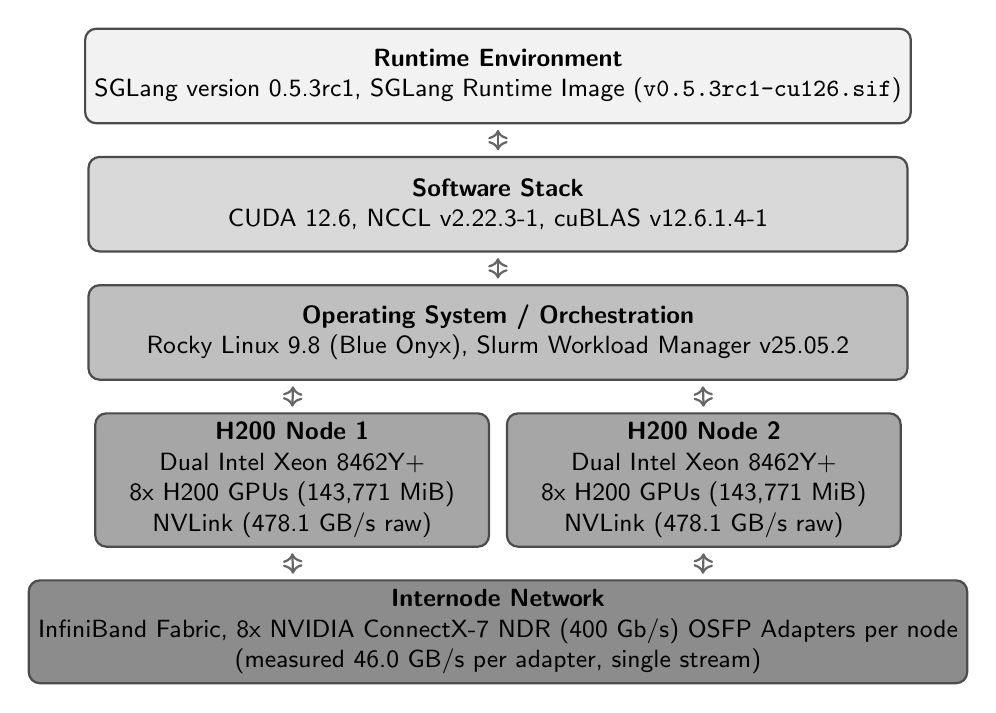
\begin{tikzpicture}[
        node distance = 0.4cm,
        box/.style = {rectangle, draw, rounded corners, minimum width=10.4cm, minimum height=1.2cm, align=center, font=\sffamily\small},
        halfbox/.style = {rectangle, draw, rounded corners, minimum width=5cm, minimum height=1.2cm, align=center, font=\sffamily\small},
        % Adjusted fill values for a bottom-to-top gradient (dark to light)
        app/.style = {box, fill=gray!10, draw=black!70, thick},
        lib/.style = {box, fill=gray!30, draw=black!70, thick},
        os/.style =  {box, fill=gray!50, draw=black!70, thick},
        hw/.style =  {halfbox, fill=gray!70, draw=black!70, thick},
        net/.style = {box, fill=gray!90, draw=black!70, thick}
    ]

    % Layer 1: Network (Bottom - Darkest)
    \node (net) [net] {\textbf{Internode Network}\\InfiniBand Fabric, 8x NVIDIA ConnectX-7 NDR (400 Gb/s) OSFP Adapters per node\\(measured 46.0 GB/s per adapter, single stream)};

    % Layer 2: Hardware (Two Nodes Side by Side)
    \coordinate (hw_center_bottom) at ([yshift=0.4cm]net.north);
    
    \node (hw1) [hw, anchor=south east, xshift=-0.1cm] at (hw_center_bottom) {\textbf{H200 Node 1}\\Dual Intel Xeon 8462Y+\\8x H200 GPUs (143,771 MiB)\\NVLink (478.1 GB/s raw)};

    \node (hw2) [hw, anchor=south west, xshift=0.1cm] at (hw_center_bottom) {\textbf{H200 Node 2}\\Dual Intel Xeon 8462Y+\\8x H200 GPUs (143,771 MiB)\\NVLink (478.1 GB/s raw)};

    % Invisible coordinate in the middle of the two nodes to align the layers above
    \path (hw1.north) -- (hw2.north) coordinate[midway] (hw_center_top);

    % Layer 3: OS & Orchestration
    \node (os) [os, above=0.4cm of hw_center_top] {\textbf{Operating System / Orchestration}\\Rocky Linux 9.8 (Blue Onyx), Slurm Workload Manager v25.05.2};

    % Layer 4: Libraries & Drivers
    \node (lib) [lib, above=of os] {\textbf{Software Stack}\\CUDA 12.6, NCCL v2.22.3-1, cuBLAS v12.6.1.4-1};

    % Layer 5: Application / Runtime (Top - Lightest)
    \node (app) [app, above=of lib] {\textbf{Runtime Environment}\\SGLang version 0.5.3rc1, SGLang Runtime Image (\texttt{v0.5.3rc1-cu126.sif})};

    % Connecting lines with bidirectional arrows
    % Bottom to Hardware
    \draw[<->, thick, shorten >=2pt, shorten <=2pt, draw=black!60] ([xshift=-2.6cm]net.north) -- (hw1.south);
    \draw[<->, thick, shorten >=2pt, shorten <=2pt, draw=black!60] ([xshift=2.6cm]net.north) -- (hw2.south);

    % Hardware to OS
    \draw[<->, thick, shorten >=2pt, shorten <=2pt, draw=black!60] (hw1.north) -- ([xshift=-2.6cm]os.south);
    \draw[<->, thick, shorten >=2pt, shorten <=2pt, draw=black!60] (hw2.north) -- ([xshift=2.6cm]os.south);

    % OS to Lib to App (Straight up the middle)
    \draw[<->, thick, shorten >=2pt, shorten <=2pt, draw=black!60] (os.north) -- (lib.south);
    \draw[<->, thick, shorten >=2pt, shorten <=2pt, draw=black!60] (lib.north) -- (app.south);

    \end{tikzpicture}
    }
    \caption{Diagram of the Network, Hardware and Software Stack}
    \label{fig:hw_sw_stack}
\end{figure}

\subsection{Network and Hardware Infrastructure}

%% Hardware/Network of Compute Nodes
All experiments were run on two Dell XE9680-F nodes of Sustainable Metal Cloud, an immersion-cooled cluster operated by Firmus in Singapore, each node with 8x NVIDIA H200 Tensor Core GPUs. Each H200 GPU had 143,771 MiB ($\approx$141 GB) of memory, idling at an average temperature of 39 degrees Celsius. Each node had two NUMA domains, with NVLink connecting the eight GPUs: 18 links per GPU at a reported 26.562 GB/s each, an aggregate 478.116 GB/s of raw unidirectional capacity per GPU (450 GB/s nominal payload bandwidth per NVIDIA's specification). Internode communication was channelled via a native InfiniBand fabric through 8x NVIDIA ConnectX-7 Single Port VPI NDR (400 Gb/s) OSFP adapters per node, running firmware version 28.41.1000. A single-stream \texttt{ib\_write\_bw} test between the nodes averaged 43,904.97 MiB/sec ($\approx$46.0 GB/s, $\approx$368 Gb/s), i.e., approximately one adapter's worth of the fabric's aggregate capacity. Each node was equipped with dual socket 32-core Intel(R) Xeon(R) Platinum 8462Y+ CPUs, with a max frequency of 4,100 MHz. Each core had 2 threads, combining to a total of 128 logical processors.

\subsection{Software Stack (Runtime Environment)}

%% OS/Software/Versions
During experimentation, the nodes' NVIDIA driver supported CUDA version 13.0; however, the SGLang runtime image\newline{} (\texttt{v0.5.3rc1-cu126.sif}), executed with Singularity \cite{kurtzer2017singularity}, utilises CUDA version 12.6. NCCL version 2.22.3-1 \cite{nccl} provided the collective communication (all-reduce, all-to-all) over RDMA. NVIDIA's linear algebra subroutines were provided by cuBLAS (version\newline{}12.6.1.4-1). Each compute node ran the Rocky Linux 9.8 operating system (Blue Onyx). A Rocky Linux 9.6 login node was used to orchestrate and queue jobs. Slurm (version 25.05.2) was utilised as the workload manager.

\subsection{Benchmark and Imposed Constraints}

The competition benchmark narrows the scope. The model architecture was confined to the DeepSeek-R1 model \cite{deepseekr1} with 671B total parameters, 37B active parameters. The nature of the task prioritised precision, and thus the data type for model weights and activations was fixed at BF16. The input dataset was the popular conversational AI benchmark dataset ShareGPT V3 \newline{} (\texttt{ShareGPT\_V3\_unfiltered\_cleaned\_split.json}) \cite{sharegpt}. The performance metric considered was total token throughput (tok/s) for offline inference. The benchmark was fixed at 2,000 prompts, with \verb|--load-format dummy| (randomly initialised weights of the correct architecture) to reduce model-load time. To ensure consistency of the generated weights between iterations, the random seed $2025$ was set. A time limit of 420 seconds was imposed, which included model loading, warm-up, and benchmarking.

\section{Results}

\subsection{Single Node Performance}
Table~\ref{tab:parallelism_configs} reports the single-node sweep of hybrid layouts occupying all eight GPUs; each layout was benchmarked twice. The maximum throughput was achieved by TP=4, DP=4, PP=2 with DP-attention enabled, whose two runs recorded 17,308.39 and 17,218.03 tok/s. A further run of this layout with \verb|--enable-torch-compile| produced the campaign best of 17,417.40 tok/s, the headline figure used throughout this paper. Its communication topology is depicted in Figure~\ref{fig:topology_1n_best}.

The dominant factor within the sweep was the DP-attention degree. Holding TP=4, PP=2 fixed, raising DP from 1 to 4 lifted throughput 44.4\%, the DP=1 layout was also the slowest configuration measured, at 11,436.32 tok/s. The alternative shape of TP=2, DP=2, PP=4, trading tensor-parallel width for pipeline depth, reached 16,498.81 tok/s at best, 4.7\% below the corresponding best hybrid sweep run.

\begin{table}[t]
  \centering
  \Description{A table displaying six configurations of Tensor, Data, and Pipeline Parallelism with their corresponding token throughput.}
  \begin{tabular}{c c c r}
    \toprule
    \textbf{TP} & \textbf{DP} & \textbf{PP} & \textbf{Throughput (tok/s)} \\
    \midrule
    4 & 4 & 2 & 17308.39 \\
    4 & 4 & 2 & 17218.03 \\
    4 & 1 & 2 & 12537.46 \\
    4 & 1 & 2 & 11436.32 \\
    2 & 2 & 4 & 16498.81 \\
    2 & 2 & 4 & 15228.52 \\
    \bottomrule
  \end{tabular}
  \caption{Comparison of different TP, DP (with DP-attention enabled when DP > 1), and PP configurations across one H200 node on SGLang. Two independent runs are shown per configuration; all sweep runs use the default scheduler parameters.}
  \label{tab:parallelism_configs}
\end{table}


\begin{figure}[t]
      \centering
      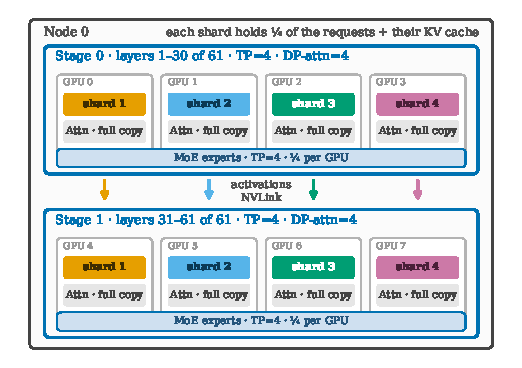
\includegraphics[width=1\linewidth]{topology_1n_best.pdf}
      \caption{Topology of communication during the forward pass for the optimal one-node configuration of \textsc{TP=4}, \textsc{DP=4}, \textsc{PP=2}. Requests are sharded across the four DP groups, eliminating KV-cache duplication, and each GPU holds a full copy of the attention weights for its layers. The first four GPUs hold the weights for layers 1--30 and the last four GPUs hold the weights for layers 31--61 of the transformer blocks. The best run of this configuration achieved 17,417.40 tok/s.}
      \label{fig:topology_1n_best}
  \end{figure} % 17,417 tok/s, one node, optimal configuration, tp = 4, dp = 4, pp=2, dp attention enabled 

\begin{figure}
      \centering
      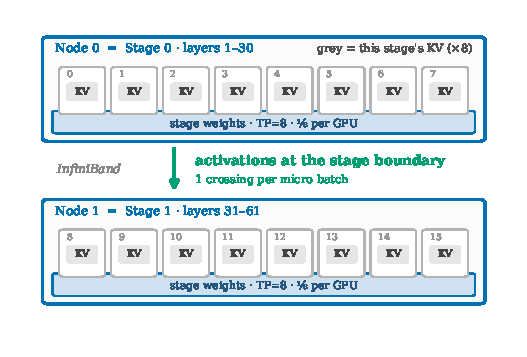
\includegraphics[width=1\linewidth]{topology_pp2.pdf}
      \caption{Topology of the two-node configuration with \textsc{PP=2}, \textsc{TP=8}, resulting in a throughput of 14,632.44 tok/s. Activations cross the InfiniBand gap once per micro-batch, at the 30--31 boundary of the 61 transformer blocks.}
       \label{fig:topology_pp2}
    \end{figure}  %% 14,632 tok/s, two nodes, pp = 2, tp = 8
      
\begin{figure}
          \centering
          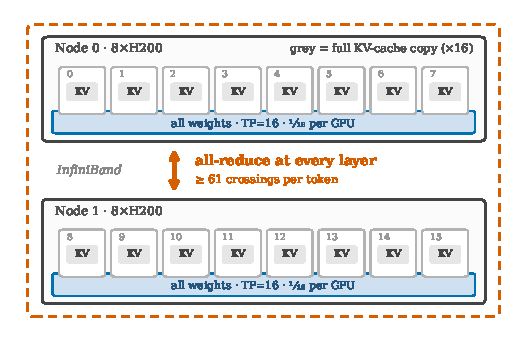
\includegraphics[width=1\linewidth]{topology_tp16.pdf}
          \caption{Topology of the two-node configuration with \textsc{TP=16}, resulting in a throughput of 11,253.39 tok/s. The KV cache is duplicated 16 times, weights are evenly distributed such that each GPU holds 1/16th of the weights, and an all-reduce occurs at every intermediate layer of the forward pass.}
          \label{fig:topology_tp16}
  \end{figure}  %% 11,253 tok/s, two nodes, tp = 16

\begin{figure}
    \centering
    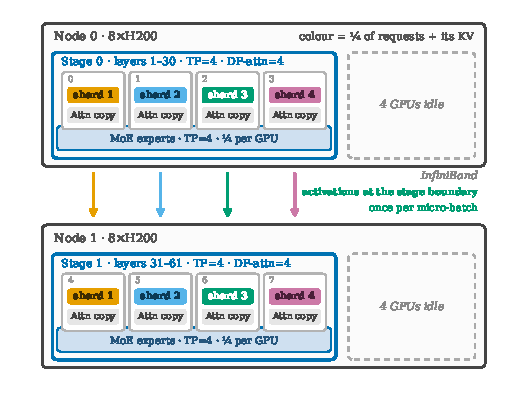
\includegraphics[width=1\linewidth]{topology_2n_best.pdf}
    \caption{Topology of the fastest two-node configuration with one shared SGLang engine (\textsc{TP=4, DP=4, PP=2}, 17,032.39 tok/s), with 4 GPUs idle on each node. Requests are sharded across the four DP groups on each node, eliminating KV-cache duplication, and each GPU holds a full copy of the attention weights for its layers. The first node's GPUs hold the weights for layers 1--30 and the second node's GPUs hold the weights for layers 31--61 of the transformer blocks.}
    \label{fig:topology_2n_best}
\end{figure} % 17,032.39 tok/s, 2 node best, tp 4, dp 4, pp 2


\begin{figure}
    \centering
    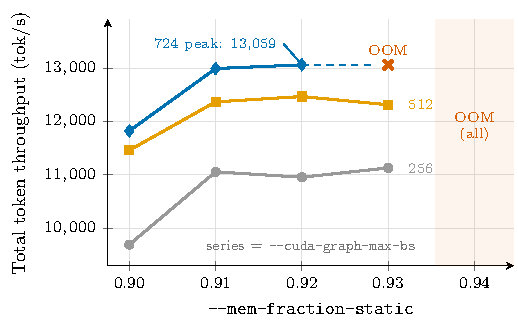
\includegraphics[width=1\linewidth]{memfrac_tuning_pgf.pdf}
    \caption{Total token throughput for the two-node \textsc{TP=16} configuration for varying \texttt{--mem-fraction-static} and \texttt{--cuda-graph-max-bs}. Throughput rises with both parameters up to the out-of-memory boundary: 0.93 fails at batch 724, and 0.94 fails at all batch sizes.}% \textcs was a typo — would fail the next compile
    \label{fig:memfracstat_bs_tuning}
\end{figure}

\subsection{Dual Node Performance}
Table~\ref{tab:twonode} summarises the two-node deployments. The strongest two-node result was the same TP=4, DP=4, PP=2 hybrid as the single-node optimum, spanned across the nodes so that the pipeline stage boundary was the only communication layer that crossed the internode fabric (Figure~\ref{fig:topology_2n_best}). It reached 17,032.39 tok/s while using only 8 of the 16 available GPUs, 2.21\% below the single-node result. No configuration that used all sixteen GPUs matched it. Of the configurations occupying all sixteen GPUs, TP=8, PP=2 was the strongest at 14,632.44 tok/s (Figure~\ref{fig:topology_pp2}), 30.0\% above TP=16, the weakest layout at 11,253.39 tok/s (Figure~\ref{fig:topology_tp16}). Tuning of the TP=16 deployment raised its peak to 13,059.21 tok/s (Figure~\ref{fig:memfracstat_bs_tuning}), still short of the TP=8, PP=2 layout, and a 40-configuration NCCL sweep produced no setting that outperformed NCCL's autotuned defaults.

Finally, we approximated serving two fully independent single-node engines, one replica per node with the 2,000 prompts split evenly between them, by benchmarking a single node on 1,000 prompts: it sustained 11,886.79 tok/s, projecting to a combined 23,773.58 tok/s across two nodes, above every configuration in which a single engine spanned both nodes. Section 5.2 discusses this projection.

\begin{table}
  \centering
  \begin{tabular}{lccccr}
    \toprule
    Deployment & TP & DP & PP & GPUs & tok/s \\
    \midrule
    Competition baseline       & 16 & 1 & 1 & 16 & 9610.57  \\
    Single engine              & 16 & 1 & 1 & 16 & 11253.39 \\
    Single engine, tuned sched.& 16 & 1 & 1 & 16 & 13059.21 \\
    Single engine              & 8  & 1 & 2 & 16 & 14632.44 \\
    Single engine              & 4  & 4 & 2 & 8  & 17032.39 \\
    Two replicas (projected)$^{\dagger}$ & 4 & 4 & 2 & 16 & 23773.58 \\
    \bottomrule
  \end{tabular}
  \caption{Comparison of two-node deployments across two H200 nodes on SGLang (DP-attention enabled when DP > 1). The GPUs column counts GPUs used by the engine; all deployments had 16 GPUs allocated. $^{\dagger}$Projected as $2\times$ a measured single-node engine given 1,000 of the 2,000 prompts (11,886.79 tok/s).}
  \label{tab:twonode}
\end{table}




\section{Discussion}
% Mention EP wasn't effective and some of the results, due to the larger scale SGLang DeepEP not being suitable for our configuration, not sure if we just put this in the limitations section...

% New Discussion Contents:
% Start with the important bit, the most efficient parallelisation across one node
% Go into multinode parallelisation, replication not distribution...
% Go into the parameter tuning that was done (mem-frac-static vs batch size)
% Go into dependency pinning & sglang optimised default versions with Singularity image
% Go into how we did the NCCL environment var sweep and how it didn't work, how good their auto tuner is.
% go into limitations (ep not being effective at small scale, DeepEP not being effective at this scale and the regular SGLang EP not being super great)

Our optimisations lifted offline throughput by 81.2\% over the official baseline (9,610.57 to 17,417.40 tok/s), or 73.2\% against the strongest of our repeats of that default configuration (10,053.70 tok/s). This discussion will outline where those gains came from, and why the largest optimisation came from refusing to distribute the engine at all.

\subsection{Most Efficient Parallelisation}
Every configuration in which per-layer collective communication crossed the internode fabric was outperformed by configurations that kept collective communication within the node. This follows from the measurements recorded in Section 3.1: intranode NVLink offers 478.116 GB/s of raw per-GPU capacity, while a single internode \texttt{ib\_write\_bw} stream measured 46.0 GB/s, roughly a $10\times$ per-flow gap, before accounting for the higher latency of the IB path. Multi-rail NCCL can stripe collectives across all eight adapters, but per-layer all-reduces are latency-sensitive and remain far more expensive over IB than over NVLink.

\textsc{TP=16} brought the most traffic onto that internode IB path: all-reduces for all 61 layers cross IB on every forward pass (Figure~\ref{fig:topology_tp16}), thus it was the weakest cross-node result at 11,253.39 tok/s, 9.6\% slower than the 12,449.13 tok/s that \textsc{TP=8} achieved on a single node with half the GPUs. Confining internode traffic to occur once per micro-batch, at the 30/31 transformer block boundary out of 61 total transformer blocks, accordingly increased the two-node throughput by 30.0\% (\textsc{TP=8, PP=2}, 14,632.44 tok/s, Figure~\ref{fig:topology_pp2}). This led us to the conclusion that if a single SGLang engine must span nodes then pipeline parallelism is the axis along which to do it.

Taken to its limit, this logic removes internode communication entirely: the best place for the stage boundary is inside a node. With all 8 GPUs on NVLink, the communication bottleneck is greatly reduced and a new bottleneck can arise, KV-cache capacity, which is why the strongest single-node configuration was not \textsc{TP=8}, but the hybrid \textsc{TP=4, DP=4, PP=2, DP-Attention Enabled} (Figure~\ref{fig:topology_1n_best}). The four DP groups shard requests and their KV cache instead of replicating it, recovering the memory that pure-TP MLA wastes on KV copies; the resulting fourfold increase in batch capacity produced a 44.4\% gain over the otherwise identical DP=1 runs (Table~\ref{tab:parallelism_configs}).

The best two-node configuration reinforces this finding: it is the same \textsc{TP=4, DP=4, PP=2} configuration spanned across the nodes so that only the 30/31 transformer block boundary crossed IB. It used just 8 of the 16 available GPUs, leaving half the GPUs on each node idle (Figure~\ref{fig:topology_2n_best}). It reached 17,032.39 tok/s, 2.21\% below the single-node result, and no configuration that used all 16 GPUs matched it. In per-GPU terms, the single-node deployment delivered $2.05\times$ the tok/s/GPU. At this model scale and with a network topology like this, less is more.

\subsection{Recommended Multi-Node Deployment: Replicate, Do Not Distribute}
These results could be misconstrued as an argument that DeepSeek-R1 should only be served from one node. This interpretation would be incorrect: we recommend serving DeepSeek-R1 from multiple nodes, each holding its own replica. This is how SGLang implements data parallelism across nodes, as multiple independent workers behind an SGLang-router instance \cite{sglangv04blog}, which distributes incoming requests under a cache-aware policy so that prefix caches stay effective across replicas. Replicas exchange nothing during the forward pass, so the internode fabric drops out of inference entirely, and combined throughput should approach twice the single-node figure ($2 \times 17{,}417.40 \approx 34{,}835$ tok/s), against 17,032.39 for the single distributed engine.

This projection is arithmetic rather than a measurement, and two effects would erode the ideal $2\times$ throughput. The first is saturation: each replica only sees half the requests, and this benchmark's fixed 2,000 prompts are not enough to keep two engines saturated. Halving the benchmark to 1,000 prompts per engine reduced the per-node throughput to 11,886.79 tok/s, or a combined 23,773.58 over two nodes, still 39.6\% above the best distributed engine but well short of the ideal. Under a genuinely saturated workload that gap should close toward $2\times$; benchmarking the two replicas simultaneously remains future work. The second is residual prefix-cache fragmentation, as the router trades cache affinity against load balance during prefix-cache maintenance. We do not measure load-balancer or HTTP-server overhead here: the offline benchmark exercises SGLang's engine and the LLM's inference steps, not a full serving deployment, and quantifying router overhead also remains future work.

\subsection{Parameter Tuning: Batch Capacity over Everything}
The saturation effect above is not incidental; it is the tuning lesson of this throughput maximisation campaign. Throughput at this scale is governed by how many requests the engine can keep in flight. DP-attention raised that ceiling by freeing KV memory; under-saturation in the 1,000-prompt experiment lowered it by starving the batch. On our default config (with \textsc{TP=16}), we swept \verb|--mem-fraction-static| and \verb|--cuda-graph-max-bs|. It was found that throughput rose with both parameters up to the OOM boundary, peaking at 13,059.21 tok/s, 16.0\% above the defaults (Figure~\ref{fig:memfracstat_bs_tuning}).

Neither tuned value transferred to the optimised parallelised configuration: \textsc{TP=4, DP=4, PP=2 with DP-attention} ran out of memory at anything above its defaults. This is the batch-capacity idea seen from the other side. Under TP=16 each GPU holds a small weight shard and the defaults leave memory idle, so there is memory that can be reclaimed by varying those parameters; the hybrid parallelism configuration holds twice the weight shard per GPU and dedicates the remainder to the DP-attention's per-group KV cache.

\subsection{Where Manual Tuning Did Not Pay: Pinned Stacks and NCCL Defaults}
We found that moving the workload from a hand-assembled virtual environment into the SGLang team's release image \newline{}(\texttt{lmsysorg/sglang:v0.5.3rc1-cu126}) increased throughput by 7.7\% (11,558.91 to 12,449.13 tok/s for the single-node \textsc{TP=8} layout)\footnote{The venv run additionally required \textsc{{-}{-}mem-fraction-static} 0.87 and \texttt{PYTORCH\_CUDA\_ALLOC\_CONF=expandable\_segments:True} to avoid out-of-memory failures; the container ran with no manual memory flags.}, and eliminated the out-of-memory instability that had required manual memory flags under the venv. This is because the image ships the current engine and the kernel stack it was tested against as one pinned artefact.

Additionally, we attempted to close the internode communication gap with software: we performed a 40-configuration sweep of NCCL parameters on the two-node \textsc{TP=16} deployment, including: \texttt{NCCL\_PROTO} (LL, LL128, Simple), \texttt{NCCL\_NTHREADS} (64--256), \texttt{NCCL\_MIN\_NCHANNELS} (4--16), GPUDirect RDMA (GDR) level, PCI relaxed ordering, and socket-thread counts. No manual configuration outperformed NCCL's defaults for that deployment (10,053.70 tok/s).

This was interpreted to mean that NCCL's internal tuner was already choosing near-optimal parameters and protocols per message size, and that manually pinning them removes that adaptability. We therefore attribute the gap to physics rather than environment or software: per-layer collectives that pay the IB path's $\sim$46~GB/s-per-rail bandwidth and higher latency cannot be configured into parity with 478~GB/s of intranode NVLink. For multi-node deployments, the remedy is to approach the problem differently and restructure the parallelism, as in Sections 5.1 and 5.2.

\subsection{Limitations and Future Work}
%**reference this shit here somewhere: https://www.lmsys.org/blog/2025-07-20-k2-large-scale-ep, and this one: lmsys.org/blog/2025-05-05-large-scale-ep***


The principal limitation is scale. With two nodes we could not reap the benefits of large-scale MoE deployments, namely prefill-decode disaggregation (PD disaggregation), where the compute-bound prefill and latency-sensitive decode can be split onto differently sized GPU pools, and large-scale expert parallelism (EP), where DeepSeek-R1's 256 routed experts can be spread thinly across many GPUs, cutting per-GPU weight memory and freeing VRAM for KV cache, increasing batch capacity, which we have shown to increase throughput. The SGLang team has reported a $5\times$ throughput improvement over vanilla tensor parallelism using large-scale distributed expert parallelism and PD disaggregation \cite{lmsysep2025}. Therefore our results should be read as a guide to throughput optimisation below the threshold where large-scale distributed EP and PD disaggregation become beneficial. Additionally, SGLang's EP consistently underperformed equivalent TP configurations on our setup, and DeepEP is designed for large scale deployments in FP8 format that our BF16 2 node setup did not fulfill.
Additionally, several constraints were placed upon the scope of our throughput maximisation campaign, most notably:
\begin{itemize}
    \item Offline throughput was the only metric used.
    \item \verb|--load-format dummy| was used, so weights were randomly initialised and expert load-balancing was not exercised.
    \item Weights were held at BF16, whereas DeepSeek-R1 is FP8 natively.
\end{itemize}

\section{Conclusion}
We present a throughput-maximisation campaign for DeepSeek-R1 over two H200 nodes, lifting offline throughput 81.2\% over the baseline (9,610.57 to 17,417.40 tok/s) through a pinned container stack, runtime compilation, and a hybrid \textsc{TP=4, DP=4, PP=2} layout with DP-attention that trades communication for KV-cache capacity. The decisive factor was interconnect locality: every configuration whose per-layer collectives crossed InfiniBand lost to one that kept them on NVLink, a penalty a 40-configuration NCCL sweep confirmed to be physical rather than software. Below the scale where wide expert parallelism pays off, our guidance is: exhaust a single node first, replicate rather than distribute across nodes, and if an engine must span nodes, span it with pipeline parallelism.


\begin{acks}
This work originated from Monash DeepNeuron's entry in the 8th APAC HPC-AI Competition, organised by the HPC-AI Advisory Council, the National Supercomputing Centre (NSCC) Singapore, and the National Computational Infrastructure (NCI) Australia. We thank NSCC Singapore for access to the ASPIRE-2A+ supercomputer and Firmus for access to the H200 cluster on which the main experiments were run. We are especially grateful to Simon Michnowicz of Monash eResearch, whose mentorship carried this work from our earliest competition preparation through to feedback on drafts of this paper. We also thank our teammates Josh Riantoputra, Giacomo Bonomi, and Isaac Barnes. Finally, we thank Pengzhi Zhu and Grace Moss for organising the competition and our participation in it.

\end{acks}

\bibliographystyle{ACM-Reference-Format}
\bibliography{base}



\end{document}
%</acmengage>